\documentclass{article}

% Language setting
% Replace `english' with e.g. `spanish' to change the document language
\usepackage[english]{babel}

% Set page size and margins
% Replace `letterpaper' with`a4paper' for UK/EU standard size
\usepackage[letterpaper,top=2cm,bottom=2cm,left=3cm,right=3cm,marginparwidth=1.75cm]{geometry}
\usepackage{caption2}
\usepackage{subfigure}
\usepackage{float}

% Useful packages
\usepackage{amsmath}
\usepackage{graphicx}
\usepackage[colorlinks=true, allcolors=blue]{hyperref}
\usepackage{ctex}
\usepackage{bm}
\usepackage{gensymb}
\renewcommand{\figurename}{图}
\renewcommand{\tablename}{表}
\newtheorem{defination}{定义}[section]
\newtheorem{theorem}{定理}[section]
\newtheorem{lemma}[theorem]{引理}
\newtheorem{corollary}[theorem]{推论}

\title{ECR离子源阅读笔记}
\author{X.Y. Wang}

\begin{document}
\maketitle

\begin{abstract}
Recent Progress in High Frequency Electron Cyclotron Resonance Ion Sources 文章阅读笔记,争取在4月1日前完成。
\end{abstract}

\section{ECRIS中的微波耦合}
尽管ECRIS已经实现了很高的性能,但是微波馈入模式仍采用很传统的设计。很多的ECRIS工作在微波波长和ECR弧腔尺寸接近的情况,比如14 GHz的常温ECRIS,它的弧腔直径是70 mm,而微波波长为20 mm。这种边界效应主导的情况下,通常认为ECR弧腔是一个多模腔,其中包含很多模式的微波。

\subsection{微观描述}
首先,我们考虑单粒子近似下,电子与高频微波的作用。热等离子体被限制在共振面内,电子沿着磁力线穿梭在两个磁镜峰之间,来回往复运动,并且在经过共振面时获得能量。
注入的微波对等离子体起到了随机加热的效应,在相互作用过程中,电子获得的能量为$\delta E = v \delta p$,此时微波损失的能量为$\hbar \omega$。于是有关系:
\begin{equation}
\delta E-\hbar\omega=0=v_\perp \delta p_\perp +v_\parallel \delta p_\parallel-\hbar\omega
\label{e1}
\end{equation}

当电子获得一个冲量$\delta p_\parallel$平行于磁力线时,微波将损失相同的动量$\hbar k_\parallel=\hbar k$。
此时公式(\ref{e1})变为
\begin{equation}
v_\perp \delta p_\perp +v_\parallel \delta p_\parallel(1-\frac{v_\phi}{v_\parallel})=0
\label{e2}
\end{equation}
其中$v_\phi=\frac{\omega}{k_\parallel}$是微波的相速度,$v_\perp$和$p_\perp$分别是电子的垂直速度和垂直动量。

如果电子的速度远小于微波的相速度,那么微波将主要改变电子垂直方向的能量。然而当电子速度远大于波速时,那么微波相互作用将变为角扩散过程,公式(\ref{e2})变为
\begin{equation}
v_\perp \delta p_\perp +v_\parallel \delta p_\parallel=0
\label{e3}
\end{equation}
但是\textbf{角扩散过程}会使电子进入到损失锥内。在ECRIS中,电子速度将小于波速,而大于波速的电子将通过损失锥丢失。

或者说,电子在沿着磁力线进行往复运动的时候,如果存在一个垂直于磁力线的电场$E$,那么电子每次经过ECR共振区时,都会获得垂直方向的冲量;如果存在一个平行于磁力线的电场,那么电子每次经过ECR共振区时,都会获得平行方向的冲量,这时电子可能会进入到损失锥里。
我们所说的平行,是指平行于轴线上的磁场,因为大量的热等离子体在轴线上产生。所以,微波是沿轴线平行入射的,产生垂直于轴线的电场。

当射频微波入射到ECRIS中,微波能量将与等离子体波进行耦合,等离子体波会将微波功率传递到ECR共振面来加热电子。

在大多数ECRIS中,真空的波长$\lambda_0$是小于等离子体的尺寸。这些等离子体波可能会参与以下作用:

\begin{enumerate}
    \item [a.]在平行传播或者准平行传播中(波矢$k$平行于磁场$B$),将存在两种情况:
    \begin{enumerate}
        \item[1.]呼啸波(电场圆极化,并且垂直于波矢$k$)$\omega_{rf}<\omega_{ce}$。在递减的磁场中,共振点为$\omega_{rf}\approx\omega{ce}$。\
        \item[2.]对于高频波,也被称为脉泽波,此时$\omega_{rf}>\omega_{ce}$,其中
        \begin{equation}
            \omega_{pe}=(\frac{n_ee^2}{\epsilon_0m_e})^{1/2}
        \end{equation}
        此时等离子体频率为$f_{pe}\approx9000\sqrt{n_e}$($f_{pe}$的单位为Hz,$n_e$的单位为cm$^{-3}$);回旋频率为
        \begin{equation}
            \omega_{ce}=\frac{eB}{m_e}
        \end{equation}
        回旋频率为$f_{ce}=28\times10^9/\text{T}$($f_{ce}$的单位为Hz)
        此时R波的频率为
        \begin{equation}
            \omega_R=\frac{(4\omega_{pe}^2+\omega_{ce}^2)^{1/2}+\omega_{ce}}{2} \text{  (right wave)}
        \end{equation}
    \end{enumerate}
    \item[b.]对于垂直或者准垂直传播的微波(波矢$k$垂直于磁场$B$):
    \begin{enumerate}
        \item [1.]O波,是电场线极化波,垂直于波矢$k$,平行于磁场$B$。
        \item [2.]X波,是电场椭圆极化波,在垂直于磁场$B$的平面内
        \begin{equation}
            \omega_{UH}=(\omega_{ce}^2+\omega_{pe}^2)^{1/2}\text{  (upper hybrid frequency)}
        \end{equation}
        \begin{equation}
            \omega_L=\frac{(4\omega_{pe}^2+\omega_{ce}^2)^{1/2}-\omega_{ce}}{2}\text{  (left wave)}
        \end{equation}
        微波在$\omega_{ce}$和$\omega_{UH}$频率下共振,在$\omega_{pe}$、$\omega_{R}$和$\omega_{L}$频率下截止。
        当$\omega_{pe}\le\omega_{rf}$时,存在ECRIS的经验公式为:
        \begin{equation}
            (I_q)_{max}\propto\omega_{rf}^2
        \end{equation}
        该公式仅适用于未激发O波时的情况。
    \end{enumerate}
\end{enumerate}
\begin{figure}[h]
    \centering
    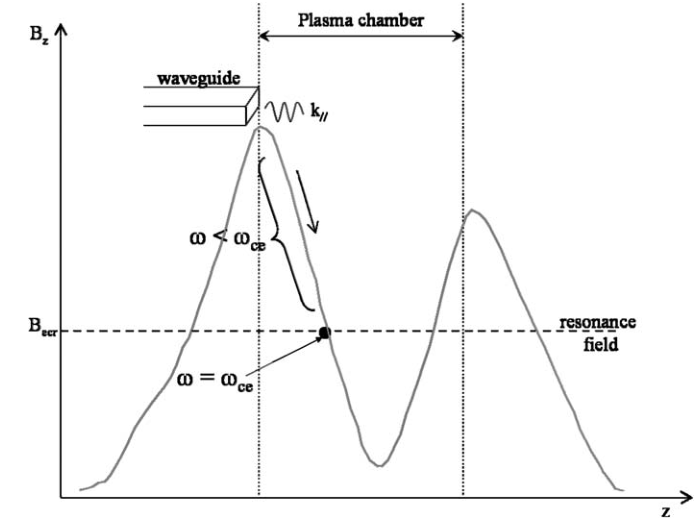
\includegraphics[width=0.5\textwidth]{magnetic beach effect.png}
    \caption{Electron cyclotron heating by transverse acceleration of electrons in a magnetic field: “magnetic beach effect.”}
    \label{f-1}
\end{figure}

考虑右旋的呼啸波,共振吸收现象发生在衰减的磁场中,也被称为磁滩(magnetic beach),这与倾斜在海滩上的水消散的情况类似。如图\ref{f-1}所示。

对于截止波,会转化为其他形式的波或者被等离子体反射,或者被部分吸收。最理想的波还是右旋呼啸波,拥有与电子回旋方向一致的右旋圆极化(RCHP)电场。这个波会将馈入的微波能量传递给共振区的电子。

由于在截止点或者被腔壁反射的微波功率可能不会被回旋共振吸收,但是也有可能通过上混杂形式共振的X波吸收$\omega_{rf}=\omega_{UH}$。

\subsection{宏观描述:本征模式}
\begin{figure}[h]
    \centering
    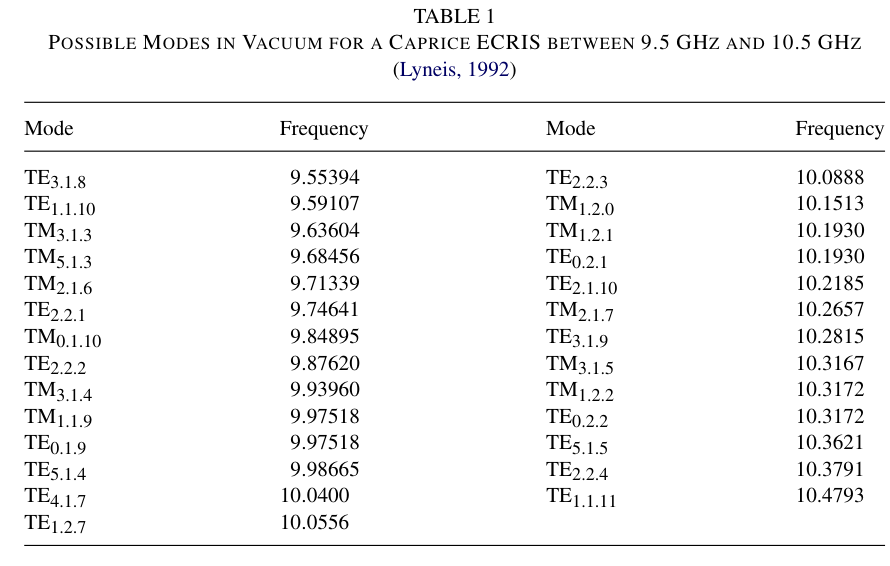
\includegraphics[width=1\textwidth]{possible modes.png}
    \caption{Caption}
    \label{f-2}
\end{figure}
ECRIS中的微波也可以被宏观描述,比如考虑等离子体腔是一个多模腔,里面可以存在许多种电磁波的模式,并且可以通过微波耦合系统选择何种模式。圆柱形腔体(ECRIS的弧腔)的本征模为$\text{TE}_{m,n,p}$或$\text{TM}_{m,n,p}$,这些角标分别代表周向$\Psi$,径向$r$,和轴向$z$。\textbf{它们实际上是相对平行的波形成的驻波},在真空中的色散关系为
\begin{equation}
    k_0^2=k_\perp^2(m,n)+k_\parallel^2(p)
\end{equation}
其中$k_0$是真空中的波数。

在理想的情况中,ECRIS中的微波耦合表现为注入的微波只有右旋波可以耦合(平行传播的呼啸波),并且在其穿过共振面时被完全吸收。

但是在真实情况中,被注入的线极化波沿主轴平行传播,然后有可以转化为呼啸波。但是只有很少的右旋波可以被吸收,左旋的微波功率则无法被完全吸收。因此大量未被吸收的微波在ECR面处被反射,随后被弧腔壁反射。所以,\textbf{等离子体的空腔模式可能存在耦合}。

让我们考虑Caprice的ECRIS,它的设计频率为10 GHz。弧腔的长度为160 mm ,直径为66 mm。计算得到它在9.5到10.5 GHz频率下的存在的模式如图\ref{f-2}所示。

尽管存在简并的微波模式,但是可以通过微波耦合系统来选择特定的模式以避免电场的简并。最好的模式为TE$_{1,n,p}$和TM$_{m,n,p}$。

\section{ECRIS中应用的耦合方案}
大多数ECRIS的弧腔尺寸仅为微波波长的几倍,等离子体体积相对于弧腔来说也十分小。\textbf{因为等离子体具有吸收性},许多本征模叠加并且在同一频率下同时存在。但是这些模式并不具有相同的权重,因此弧腔中的电磁场分布主要取决于耦合系统的选择。
\subsection{频率超过20 GHz}
\begin{figure}
    \centering
    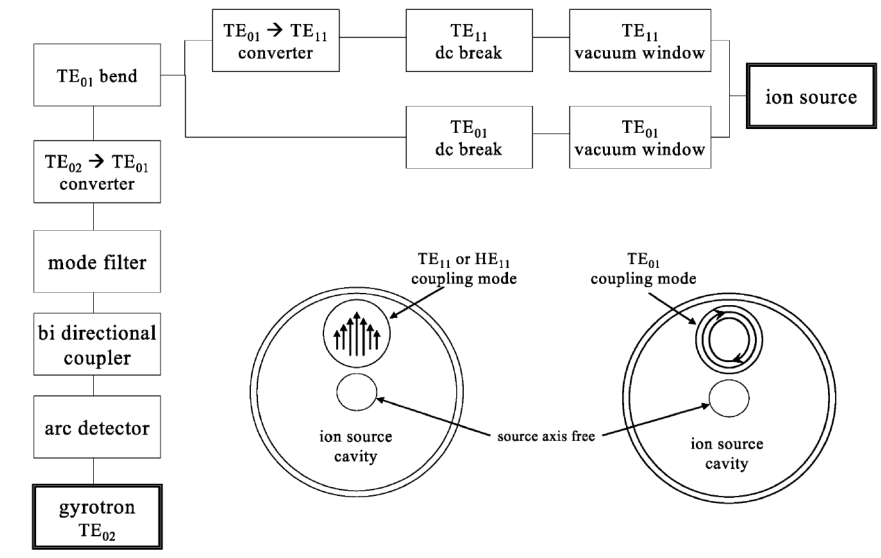
\includegraphics[width=0.8\textwidth]{Schematic diagram.png}
    \caption{Schematic diagram of a 28 GHz transmission line with two coupling possibilities
(arrows indicate the electric field).}
    \label{f-3}
\end{figure}
当微波频率在20 GHz以下时,常常采用矩形波导进行微波传输。但是超过20 GHz后,高功率微波源常常采用回旋管,它的输出常为圆波导或者准光学传输,比如28 GHz微波采用TE$_{02}$的过尺寸波导。从微波源到离子源的微波传输线必须经过严格的计算和设计,以避免传输过程中出现模式转换而导致的微波损失。这些杂散的模式由于波导制作的不完美导致的,比如倾斜、弯曲、直径变化、高压绝缘和真空窗等。如图\ref{f-3}所示为28 GHz微波传输线。它可以提供两种微波馈入方式。在回旋管微波窗处安装了一个弧光探测器,用以防止打火对回旋管造成损伤。两个功率计分别测量输出功率和反射功率。模式过滤器用来过滤所有超过TE$_{02}$的模式,随后TE$_{02}$模式转化为TE$_{01}$模式,因为TE$_{01}$模式在长距离的传输中有更小的欧姆损失。随后TE$_{01}$模式可以转化为TE$_{11}$或HE$_{11}$模式,然后通过绝缘传输线馈入ECRIS中。

在传输线中,波导的弯头是一个非常重要的器件,因为相速度接近的模式之间转换,通常发生在具有轴向曲率的过尺寸波导中。DC-break通常采用叠片铝和聚四氟乙烯环做成的半周期结构。

在核聚变研究中超过30 GHz频率的微波通常采用准光学方式。

\subsection{总结}
通常来说,在设计像ECRIS这样的设备时很难适应理论,特别在设计微波辐射器时,比如在径向上留出空间放置波导就会减弱径向的磁场约束。幸好ECRIS是一个多模腔,并且具有很复杂的磁场可以使电子在腔中总有可以获得横向能量的地方。但是入射的微波功率,几乎有一半通过不同的方式被损失:
\begin{enumerate}
    \item [1.]损失在波导和匹配系统中;
    \item [2.]进入到损失锥中的电子;
    \item [3.]反射功率;
    \item [4.]损失在腔壁上。
\end{enumerate}

ECRIS中总共的吸收功率可以写为:
\begin{equation}
    P_{abs}\approx\frac{n_ekT_eV}{\tau_e}
\end{equation}
其中$\tau_e$是电子的约束时间,$V$是热等离子体体积。

为了有效的传输和耦合微波功率到ECRIS中,需要在设计微波传输线时特别注意以最小化损耗。当超过1kW的微波功率时,十分推荐使用过尺寸的波导管。但是波导的位置需要特别小心的选取,以防止寄生共振造成的出气效应。

一旦等离子体被产生,对电子和离子密度和温度的诊断尤为重要。



































\clearpage

\begin{table}
\centering
\begin{tabular}{l|r}
Item & Quantity \\\hline
Widgets & 42 \\
Gadgets & 13
\end{tabular}
\caption{\label{tab:widgets}An example table.}
\end{table}

\bibliographystyle{alpha}
\bibliography{sample}

\end{document}